\subsection{SqlClient}
Die \eigenName{SqlClient} Klasse verwaltet die Verbindung zum \ac{sql} Server. \\Auf dem \ac{sql} Server sind alle Daten gespeichert, die persistiert werden müssen. 
Das Klassendiagramm der \eigenName{SqlClient} Klasse ist in \refFig{fig:backend:classDiag:SqlClient} dargestellt.
Die Klasse bedient sich dabei der offiziellen Bibliothek \eigenName{MariaDB Connector/C API} der OpenSource Datenbank-Engine MariaDB \citep{mariaDB}.
\begin{figure}[ht]
  \centering
  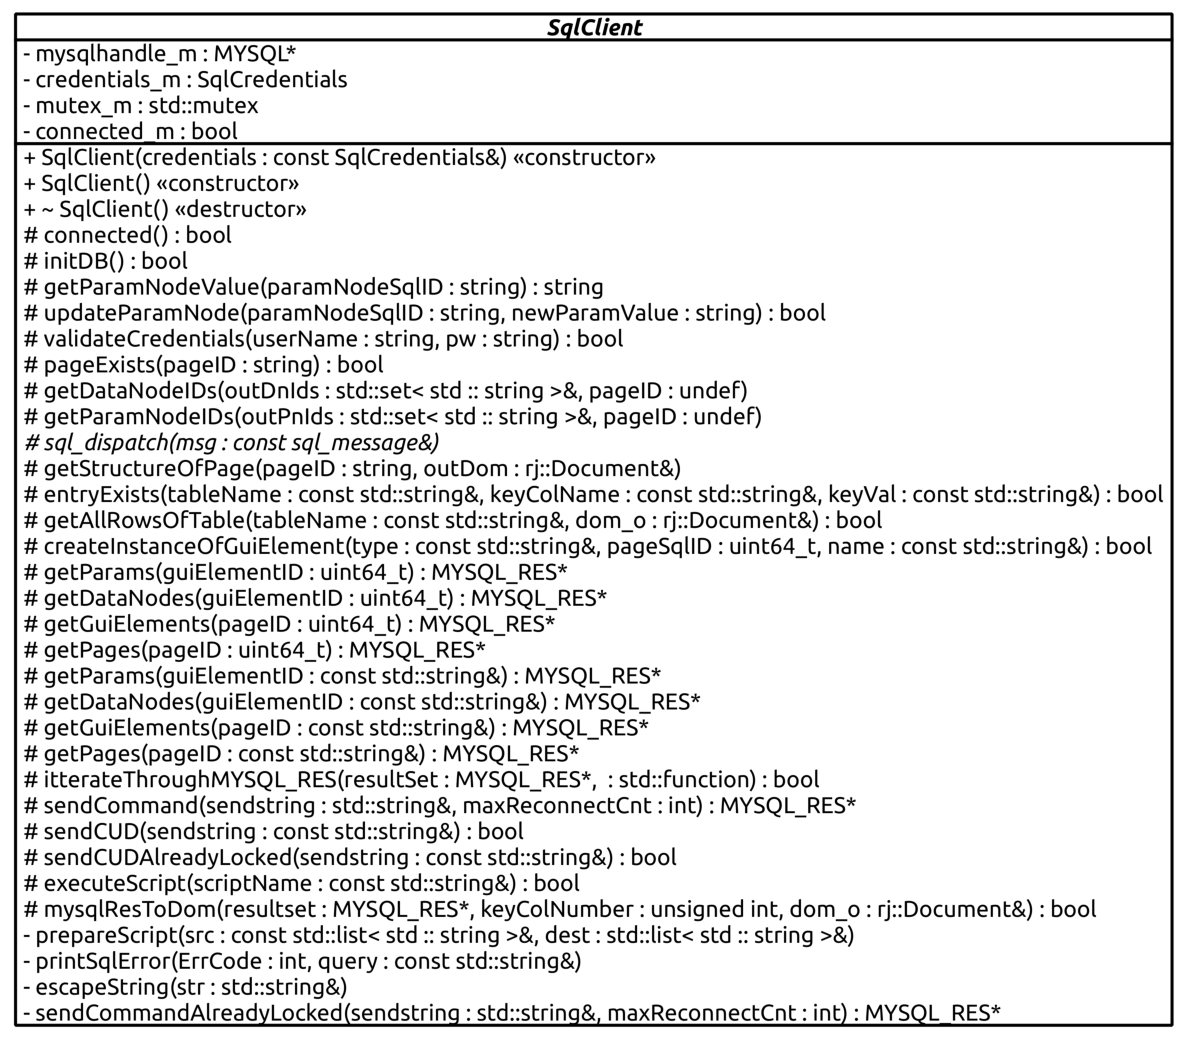
\includegraphics[width=\textwidth]{content/hauptteil/umsetzungPoC/backend/uml/classesOfOverview/SqlClient.pdf}
  \caption{Klassendiagramm der Klasse \eigenName{SqlClient}}
  \label{fig:backend:classDiag:SqlClient}
\end{figure}
Die Datenstruktur des Servers ist in Abschnitt \ref{subsec:dataBackend} beschrieben und dort in \refFig{img:erd} dargestellt.
Diese Struktur ist auf dem \ac{sql} Server vorhanden und wird durch das Skript in \refList{list:createSqlTables} auf dem externe Server konstruiert.
Die \eigenName{SqlClient} Klasse kann mit der Methode \eigenName{executeScript} ein \ac{sql} Skript als Datei ausführen, indem sie es in einzelne Querys zerteilt und diese dann einzeln an den Server sendet.
Das Zerteilen eines Skript und das Vorbereiten zur Ausführung ist in der Methode \eigenName{prepareScript} implementiert. 
Beim Testen der Methode hat sich herausgestellt, dass diese Funktionalität der \eigenName{sql} Client Klasse Skripte auszuführen, schwieriger zu implementieren ist als anfangs vermutet.
Dies liegt daran, dass das Definieren von \emph{stored Procedures} (siehe Abschnitt \ref{subsec:storedProc}) es nötig macht das Semikolon als Trennzeichen zu ändern, 
da in einem Query der Quellcode vorhanden ist, der selbst aus mehreren Querys besteht, die mit einem Semikolon getrennt sind.
Ist ein Skript vorbereitet, so können die einzelnen Querys des Skripts durch den Aufruf der Methode \eigenName{sendCUD} auf dem Server ausgeführt werden.
Die Methode \eigenName{sendCUD} bedient sich dabei der Methode \eigenName{sendCommand}, die die Query an den Server weiterleitet.
Da die Verbindung zum \ac{sql} Server eine geteilte Ressource ist, ist der Zugriff darauf durch \eigenName{sendCommand} durch ein Mutex geschützt, sodass immer nur ein Thread gleichzeitig ein Query senden kann.
Die Klasse \eigenName{SqlClient} bietet viele Methoden um die Daten in der Datenbank abzufragen oder zu verändern.
Um Daten abzufragen werden meistens Querys ausgeführt, die mit \eigenName{Select} beginnen.
Allerdings sind ein paar komplizierte Querys in \emph{stored Procedures} auf dem Server ausgelagert.
Die Prozeduren werden durch das Skript \eigenName{createProcedures} (siehe Anhang \refList{list:createProcedures}) erzeugt.
Um ein \ac{gui} Element zu instanzieren, sind eine Menge an Operationen notwendig.
Diese Operationen sind auch als Prozeduren implementiert und werden durch eine einfache \eigenName{Call} Query aufgerufen.
Immer wenn der Wert einer \emph{ParamNode} auf dem \ac{sql} Server durch Aufruf der Methode \eigenName{updateParamNode} geändert wird, werden alle verbunden \eigenName{ws\_session} Objekte darüber informiert.
Diese Funktionalität ist implementiert, indem in der \eigenName{updateParamNode} Methode zuerst geprüft wird, ob die Änderung tatsächlich eine Änderung darstellt, oder ob der Wert bereits dem neuen Wert entspricht.
Ist das der Fall, wird versucht den Wert auf dem \ac{sql} Server zu ändern. War die Änderung erfolgreich, wird ein \eigenName{sql\_message} Objekt (siehe Klassendiagramm in \refFig{fig:backend:classDiag:sqlMsg}) erstellt 
und der Methode \eigenName{sql\_dispatch} der Klasse \eigenName{SqlClient} übergeben. 
\begin{figure}[ht]
  \centering
  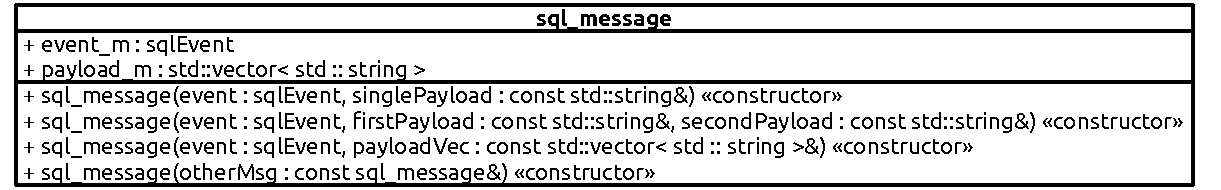
\includegraphics[width=\textwidth]{content/hauptteil/umsetzungPoC/backend/uml/classesOfOverview/sql_message.pdf}
  \caption{Klassendiagramm der Klasse \eigenName{sql\_message}}
  \label{fig:backend:classDiag:sqlMsg}
\end{figure}
Die Datenstruktur des \eigenName{sql\_message} Objekts ist dabei ähnlich aufgebaut wie die des \eigenName{ws\_message} Objekts.
Es besitzt ein Event und ein Payloadvektor.
Die Methode \eigenName{sql\_dispatch} ist in der Klasse \eigenName{Backend} reimplementiert und reagiert auf das \eigenName{sql\_message} Objekt je nach Event.
In diesem Fall ist das Event \eigenName{paramNodeChange}. Hier wird der Payloadvektor so interpretiert, dass das erste Element die NodeID ist und das zweite der neue Wert.
Diese Information wird dann schließlich als \eigenName{ws\_message} kodiert und die Methode \eigenName{publishToAllSessions} der \eigenName{WebsocketServer} Klasse aufgerufen, 
welche diese Information dann an alle Sessions weiterleitet.
In jeder Methode, in der Daten der Websocket Schnittstelle in Querys verwendet werden, können diese nicht als \mintinline{c++}{const std::String&} übergeben werden, da diese durch die Methode \eigenName{escapeString} verändert werden um eine \emph{SQL-Injection} vorzubeugen.
Diese Methode bedient sich dazu einer entsprechenden Funktion der verwendeten Bibliothek.
Würde die Referenz auf den String als \mintinline{c++}{const} übergeben werden, könnte die Methode den String nicht verändern.

%kurze Erwähnung sinn der klasse
%datenaustausch zwischen SqlClient zu abgeleitetrer...(dispatcher.... ) (I/O)

%beschreibung msg klasse mit diagram

%dispatcher codeausschnitt
%beschreibung dispatcher